%!TEX root = ../../Main.tex
\graphicspath{{Chapters/Test/}}
%-------------------------------------------------------------------------------


\section{I2C kommunikation}
Til at starte med havde gruppen ikke planer om at inkorporere I2C i NSS, da den simple løsning var at have både TFT skærmen og Color Sensoren sat til samme Arduino. Dette viste sig ikke at kunne lade sig gøre, da skærmen og sensoren delte nogle pins, hvilket gjorde at systemet ikke fungerede. Desværre kunne vi ikke bruge andre pins til sensoren, da de to pins der er at vælge imellem begge sad i vejen for skærmen. Derfor valgte gruppen at splitte systemet op og anvende I2C. På grund af denne ekstra arbejsbyrde, blev SD kort implementationen nedprioriteret.



\subsection{I2C master}
Masteren blev valgt implementeret på TFT display modulet, da det ikke ville give mening at lade sensor modulet sende kommandoer til display modulet. Istedet for sendes der en char fra slaven, som repræsenterer en farve.

Til udviklingen af masteren har et timing diagram over I2C protokollen, se \autoref{fig:I2CTIming}, været utrolig nyttig. Det er på baggrund af dette diagram gruppen har lavet både master og slave. I masterens tilfælde skal den forst initieres. Det sker ved at sætte bestemte dataregistre rigtigt. Først bestemmer man hvilken clock SCL skal have. SCL kan udregens på følgende måde:

\begin{equation}
SCL clock freq = \frac{CPU clock freq}{16+2(TWBR)*4^{TWPS}} 
\end{equation}



Dette gøres i TWSR registeret, ved at vælge hvad prescaleren skal være på. 

\begin{figure}[H]
	\centering
	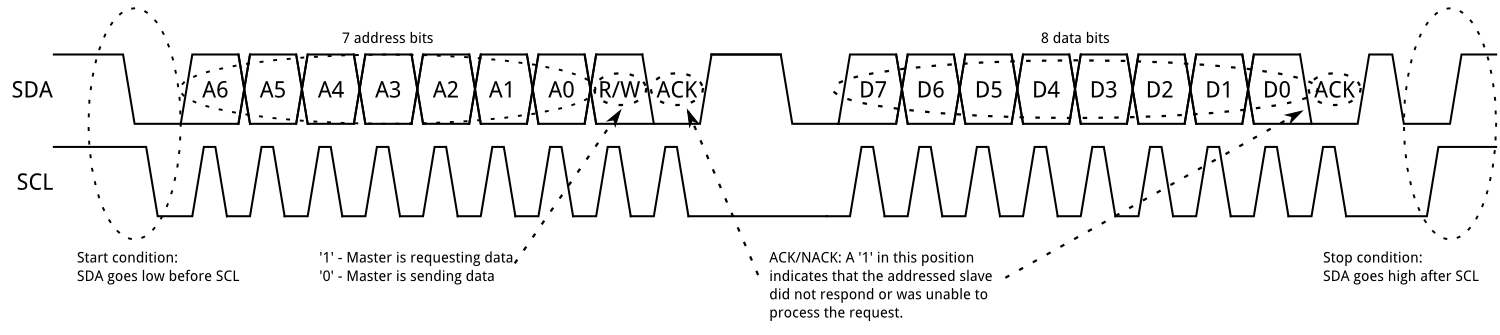
\includegraphics[width = 450pt]{Img/I2CTiming.png}
	\caption{I2C timing diagram}
	\label{fig:I2CTIming}
\end{figure}

Masteren er derfor sat op som en recieving master, hvilket vil sige at den kun modtager data fra slaven.





\subsection{I2C slave}



